\begin{frame}{Результати роботи}
	\framesubtitle{Випадок центрального розташування}
	\manimate
	В роботі було отримано точну аналітичну формулу максимальної кількості автомобілів $F(X)$ на паркінгу довжини $X$ у випадку центрального розташування.
	\begin{block}{Теорема 1}
		У випадку вибору місця для автомобіля в центрі вільного проміжку максимальна кількість автомобілів $F(X)$ на паркінгу визначається наступним чином
		\[
			F(X) = 2^k - 1,\; \text{якщо } X \in [2^k - 1, 2^{k+1} - 1), k \in \mathbb{N} \cup \{0\}.
		\]
	\end{block}
	\note{Тут треба пояснити, що центральне розташування – коли автомобілі стають посерелині вільного проміжку, згадавши останню картинку поперелнього слайда, і швиденько перейти на наступний слайд, де є гарний графік.}
\end{frame}

\begin{frame}{Результати роботи}
	\framesubtitle{Випадок центрального розташування}
	\manimate
	\vspace{-10pt}
	\begin{figure}
		\centering
		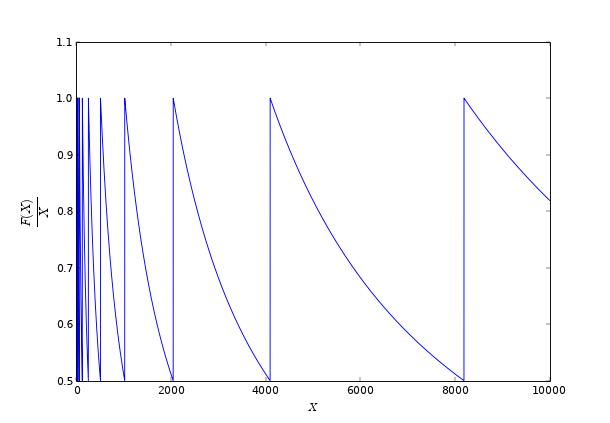
\includegraphics[width=0.65\linewidth]{central_placer}
		\caption{\centering Графік відношення $F(X)/X$ у випадку центрального розташування}
	\end{figure}
	\note{Цей випадок є яскравим прикладом того, що асимптотична поведінка не завжди має місце.}

%%%%%%%%%%%%%%%%%%%%%%%%%%%%%%%%%%%%%%%%
	
\end{frame}
\begin{frame}{Результати роботи}
	\framesubtitle{Випадок рівномірного розташування}
	\manimate
	В роботі було виведене інтегральне рівняння зі зсувом для математичного сподівання $m(X)$ максимальної кількості автомобілів на паркінгу довжини $X$.
	\begin{block}{Теорема 2}
	У випадку розташування автомобілів за рівномірним розподілом виконується наступне співвідношення для $m(X)$:
        \[
            	m(X + 1) = \frac{2}{X} \int\limits_0^{X} m(t) dt + 1,\quad \forall X > 0
        \]
	\end{block}
\end{frame}

\begin{frame}{Результати роботи}
	\framesubtitle{Випадок рівномірного розташування}
	\manimate
	\begin{block}{Теорема 2 (продовження)}
		До того ж, має місце асимптотична поведінка
		\[
	m(X) \sim  \kappa  \cdot X, \quad X \rightarrow \infty.
		\]
		де
		\[
			\kappa = \int\limits_0^\infty \exp\left( -2\int\limits_0^s \frac{1 - e^{-\tau}}{\tau} d\tau  \right) ds 
		\]
	\end{block}
	\note{На основі інтегрального рівняння було отримано асимптотику математичного сподівання $m(X)$ максимальної кількості автомобілів на паркінгу довжини $X$ при $X \rightarrow \infty$.}
\end{frame}

\begin{frame}{Результати роботи}
	\framesubtitle{Випадок рівномірного розташування}
	\manimate
	Приблизне значення сталої $\kappa$ може бути отримано чисельними методами:
	\[
		\kappa \approx 0.747598.
	\]
	На практиці було проведене імітаційне моделювання парковки за моделлю рівномірного розташування, і було отримане експериментальне значення для $\kappa$:
	\[
		\kappa^{experimental} = \frac{\#cars}{lenght} = 0.747588.
	\]
	\note{Порівняти результати аналітичної формули та імітаційного моделювання.}
\end{frame}

%%%%%%%%%%%%%%%%%%%%%%%%%%%%%%%%%%%

\begin{frame}{Результати роботи}
	\framesubtitle{Випадок суміші рівномірного та розподілу Бернулі}
	\manimate
	В роботі було виведене інтегральне рівняння зі зсувом для математичного сподівання $m_\alpha(X)$ максимальної кількості автомобілів на паркінгу довжини $X$.
	\begin{block}{Теорема 3}
	У випадку розташування автомобілів за сумішшю рівномірного розподілу та розподілу Бернуллі виконується наступне співвідношення для $m_\alpha(X)$:
        \[
		m_\alpha(X + 1) = 1 + \alpha m(X) + \frac{2(1-\alpha)}{X} \int\limits_0^{X} m(t) dt,\quad \forall X > 0
        \]
	\end{block}
\end{frame}

\begin{frame}{Результати роботи}
	\framesubtitle{Випадок суміші рівномірного та розподілу Бернулі}
	\manimate
	\begin{block}{Теорема 3 (продовження)}
		До того ж,
		\[
	m(X) \sim  \kappa_\alpha \cdot X
		\]
		де
		\[
			\kappa_\alpha = \frac{1}{1-\alpha}  \int\limits_0^\infty \exp\left( -2\int\limits_0^s \frac{e^{\tau} - 1}{\tau(e^\tau - \alpha)} d\tau  \right) ds 
		\]
	\end{block}
	\note{На основі інтегрального рівняння було отримано асимптотику математичного сподівання $m_\alpha(X)$ максимальної кількості автомобілів на паркінгу довжини $X$ при $X \rightarrow \infty$.}
\end{frame}

\begin{frame}{Результати роботи}
	\framesubtitle{Випадок рівномірного розташування}
	\manimate
	Приблизне значення сталої $\kappa_\alpha$ може бути отримано чисельними методами:
\begin{table}
	\centering
	\scriptsize
\begin{tabular}{|p{0.1\textwidth}|p{0.1\textwidth}|p{0.1\textwidth}|p{0.1\textwidth}|p{0.1\textwidth}|p{0.1\textwidth}|}
	\hline
	$\alpha$ & 0 & 0.1 & 0.2 & 0.3 & 0.4 \\
	\hline
	$\kappa_\alpha$ & 0.747598 &0.76351 &0.780574 &0.798962 &0.818896  \\
	\hline
	\hline
	$\alpha$  & 0.5 & 0.6 & 0.7 & 0.8 & 0.9\\
	\hline
	$\kappa_\alpha$  &0.84066 &0.864638 &0.891365 &0.92165 &0.956849 \\
	\hline
\end{tabular}
\end{table}

	На практиці було проведене імітаційне моделювання парковки за моделлю рівномірного розташування, і було отримане експериментальне значення для $\kappa_\alpha$:
\begin{table}
	\centering
	\scriptsize
\begin{tabular}{|p{0.1\textwidth}|p{0.1\textwidth}|p{0.1\textwidth}|p{0.1\textwidth}|p{0.1\textwidth}|p{0.1\textwidth}|}
	\hline
	$\alpha$ & 0 & 0.1 & 0.2 & 0.3 & 0.4 \\
	\hline
	$\kappa_\alpha$ & 0.747588 &0.76352 &0.780569 &0.798959 &0.818891  \\
	\hline
	\hline
	$\alpha$  & 0.5 & 0.6 & 0.7 & 0.8 & 0.9\\
	\hline
	$\kappa_\alpha$  &0.84055 &0.863658 &0.891214 &0.92158 &0.95693 \\
	\hline
\end{tabular}
\end{table}
	\note{Порівняти результати аналітичної формули та імітаційного моделювання.}
\end{frame}


%%%%%%%%%%%%%%%%%%%%%%%%%%%%%%%%%%%%%%%%%%%%%

\begin{frame}{Результати роботи}
	\framesubtitle{Моделювання двовимірної парковки}
	\manimate
	Було проведено імітаційне моделювання для двовимірного прямокутного паркінгу з моделлю розташування автомобілів за рівномірним розподілом. Отримали наступні результати:
\begin{table}
	\centering
\begin{tabular}{|cc|c|}
	\hline
	 $a$ & $b$ & $\frac{\#cars}{a*b}$ \\
	 \hline
	 50 & 50 & 0.5801 \\
	 50 & 100 & 0.5889 \\
	 100 & 100 & 0.5951 \\
	 50 & 200 & 0.5975 \\
	 200 & 200 & 0.6021 \\
	 500 & 500 & 0.6111 \\
	\hline
\end{tabular}
\end{table}
	\note{Цей додаток було створено для більш реалістичного моделювання процесу паркування у випадку двовимірної парковки. Найбільш цікавою характеристикою є математичне сподівання відношення максимальної кількості автомобілів, отриманого внаслідок ітерацій імітаційного моделювання, до загальної площі прямокутної парковки. Існує гіпотеза Паласті, яка стверджує, що ця характеристика прямує до $\kappa^2 \approx 0.56$. На жаль, вона не підтверджується практично.}
\end{frame}

